\documentclass{beamer}

\usepackage{beamerthemesplit}

\usetheme{Pittsburgh}
\usecolortheme{seagull}

\usefonttheme{serif}

\title{Shear Estimation}
\author
{
    Erin Sheldon \\
    Brookhaven National Lab
}

\begin{document}

\frame{\titlepage}

\section{Introduction}


\frame
{
    %\fontsize{10}{<value for \baselineskip>}\selectfont
    \fontsize{10}{\baselineskip}

    \frametitle{Gravitational Shear}

    \begin{columns}

        \begin{column}{0.5\textwidth}

            \begin{itemize}
                \item The path of light appears curved as it passes massive objects
                \item The ``deflection'' differs across the face of an extended source galaxy.
                \item Shear distorts the image; we say it's ``shape'' is altered.
                \item Galaxies are already elliptical, but shear produces spatial shape correlations.
                    Shape correlations are closely related to mass density
                    correlations.

            \end{itemize}
        \end{column}
        \begin{column}{0.5\textwidth}
            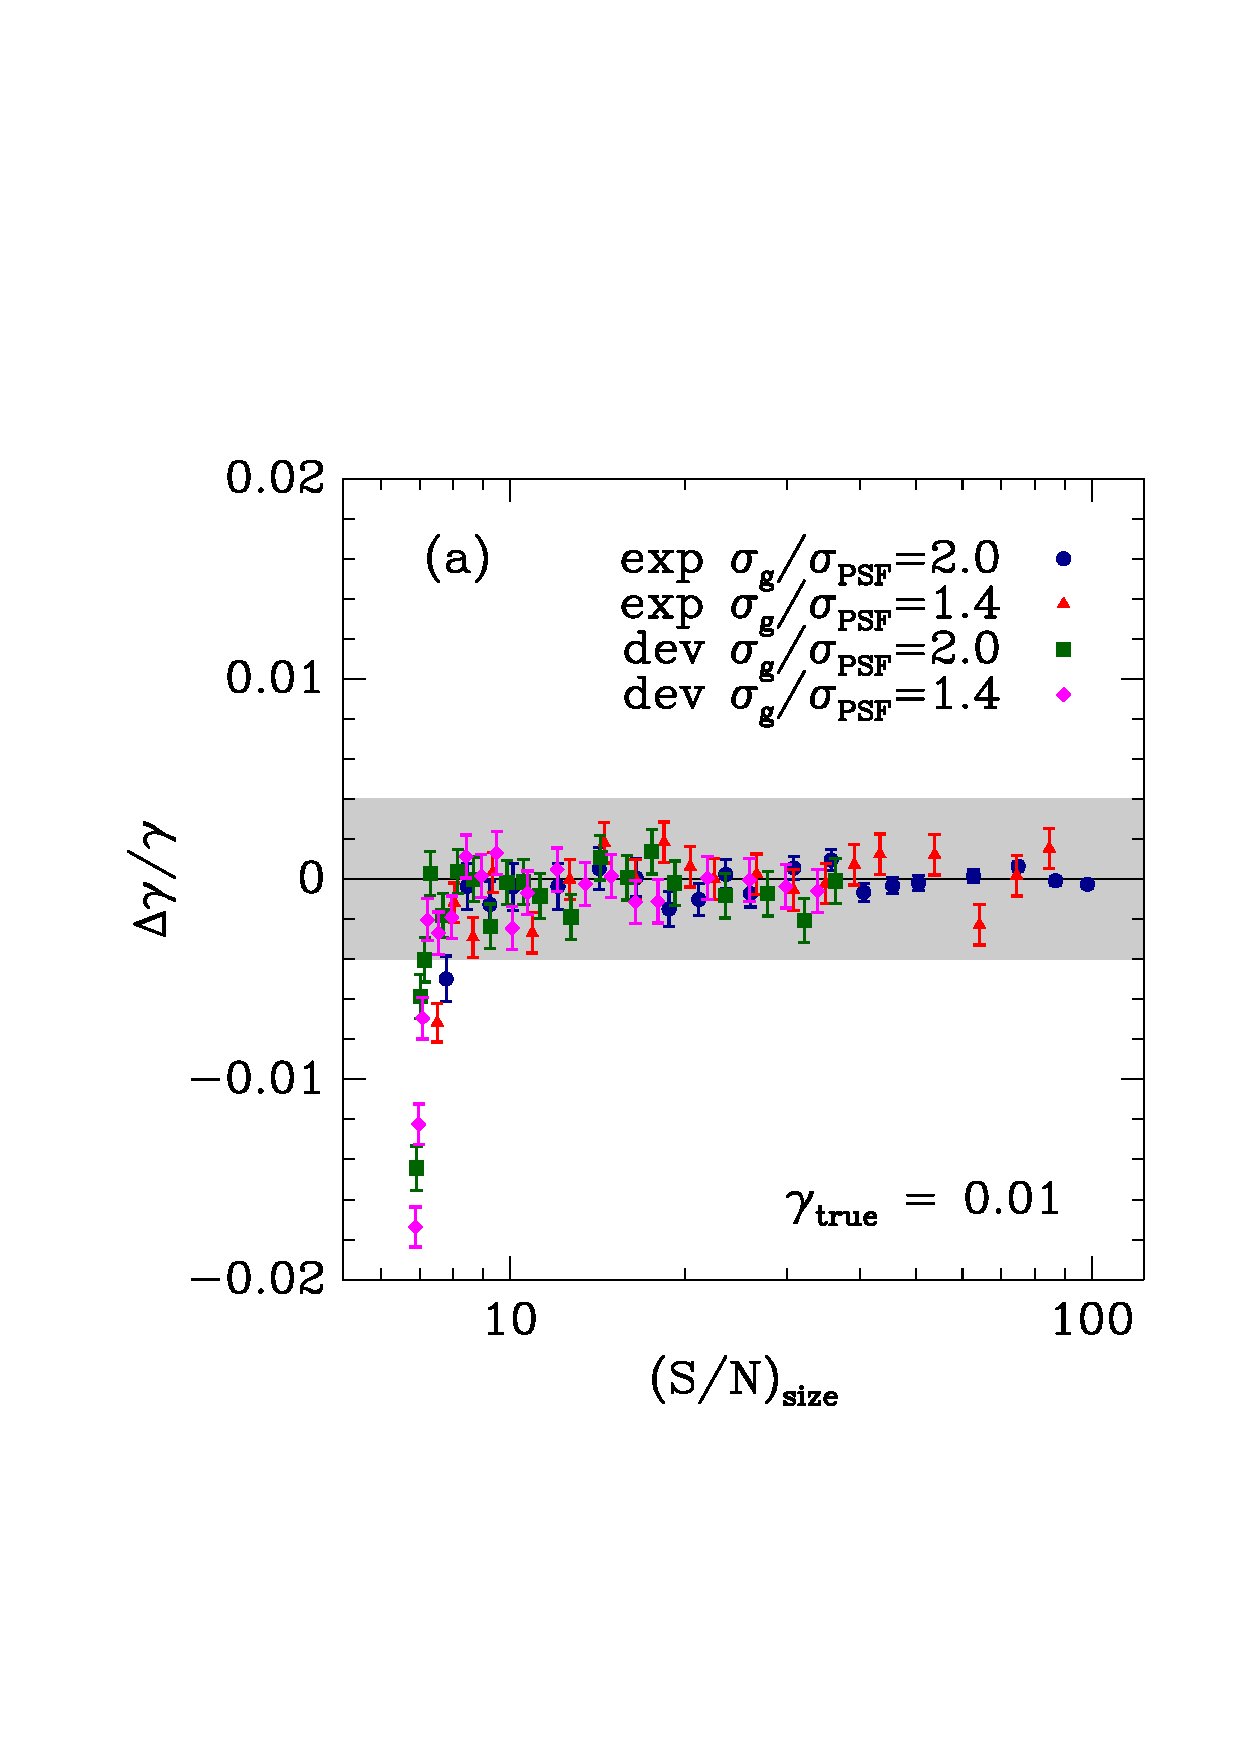
\includegraphics[width=\textwidth]{cbafit-geg-T-s2n.pdf}
        \end{column}
    \end{columns}
}



\frame
{
    \frametitle{Measuring Shear}

    \begin{itemize}
        \item For a perfect detector with no noise, just measure
            the second moments and look for the correlations.
        \item The atmosphere, telescope, and instrument smear
            the image: the Point Spread Function (PSF).
        \item That just adds to the moments, so we just need to
            subtract off the PSF moments!
        \item But we have noise, so the moments don't converge.
    \end{itemize}
}

\frame
{
    \frametitle{PSF and Noise}
    
    \begin{itemize}

        \item One can use a weight function to suppress the noise, but then we
            need to derive how that measurement responds to smearing by the PSF
            and shearing (e.g. Kaiser, Squires, \& Broadhurst, Bernstein \& Jarvis, Melchior,
                    Bernstein \& Armstrong)

        \item Alternatively, one can forward-model the problem: fit a model that is
            convolved with an estimate of the PSF.  Limited by how well one can
            model the galaxy and PSF (e.g. Miller et al., Bernetein \& Armstrong).

    \end{itemize}
}




\end{document}
